\documentclass[10pt]{article}
\usepackage[margin=15mm]{geometry}
\usepackage{amsmath,amssymb,tikz,pgfplots}
\pgfplotsset{compat=1.18}
\definecolor{digitZero}{HTML}{246C91}
\definecolor{digitOne}{HTML}{BC632E}
\pagestyle{empty}
\begin{document}
\begin{center}
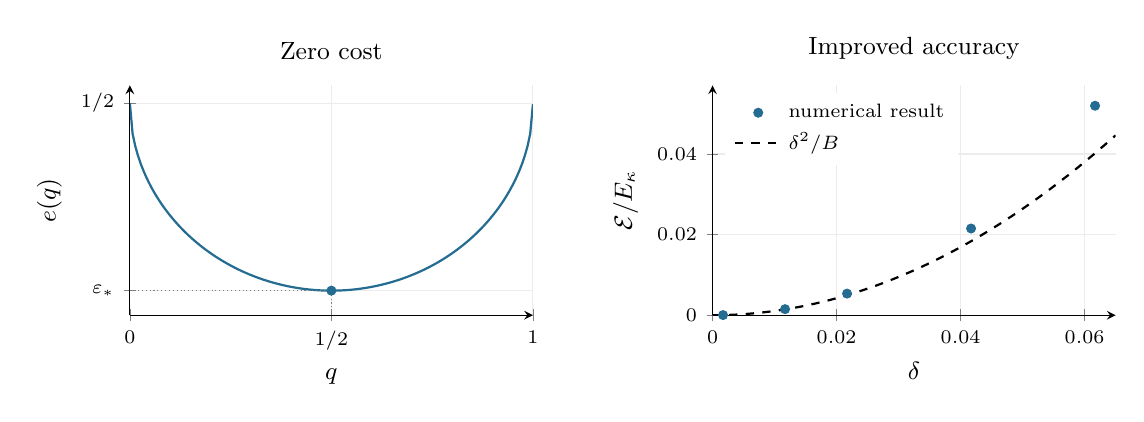
\begin{tikzpicture}
\begin{axis}[width=6.7cm,height=4.5cm,scale only axis=false,
 axis lines=left,tick label style={font=\scriptsize},label style={font=\small},
 title style={font=\small},legend style={font=\scriptsize,draw=none,fill=white},
 legend cell align=left,scaled ticks=false,grid=major,grid style={gray!15},
 tick label style={/pgf/number format/use period,/pgf/number format/fixed,/pgf/number format/precision=3,font=\scriptsize},xmin=0,xmax=1,ymin=.14,ymax=.53,
 xlabel={$q$},ylabel={$e(q)$},title={Zero cost},xtick={0,.5,1},
 xticklabels={$0$,$1/2$,$1$},ytick={.181690113816,.5},yticklabels={$\varepsilon_*$,$1/2$}]
\addplot[digitZero,thick,domain=0:1,samples=151] {.5-2/pi*sqrt(max(0,x*(1-x)))};
\addplot[gray,densely dotted] coordinates {(.5,.14) (.5,.181690113816) (0,.181690113816)};
\addplot[only marks,mark=*,mark size=1.6pt,digitZero] coordinates {(.5,.181690113816)};
\end{axis}
\begin{axis}[width=6.7cm,height=4.5cm,scale only axis=false,
 axis lines=left,tick label style={font=\scriptsize},label style={font=\small},
 title style={font=\small},legend style={font=\scriptsize,draw=none,fill=white},
 legend cell align=left,scaled ticks=false,grid=major,grid style={gray!15},
 tick label style={/pgf/number format/use period,/pgf/number format/fixed,/pgf/number format/precision=3,font=\scriptsize},at={(7.4cm,0)},anchor=south west,
 xmin=0,xmax=.065,ymin=0,ymax=.057,xlabel={$\delta$},ylabel={$\mathcal E/E_\kappa$},
 title={Improved accuracy},xtick={0,.02,.04,.06},ytick={0,.02,.04},legend pos=north west]
\addplot[only marks,mark=*,mark size=1.6pt,digitZero] coordinates {(0.00169011381621,3.03269011296e-05) (0.0116901138162,0.0015011867754) (0.0216901138162,0.00536049680095) (0.0416901138162,0.0215052847179) (0.0616901138162,0.0519592518471)};
\addlegendentry{numerical result}
\addplot[black,dashed,thick,domain=0:.065,samples=101] {x^2/(.5-4/pi^2)};
\addlegendentry{$\delta^2/B$}
\end{axis}
\end{tikzpicture}
\end{center}\end{document}
